\subsection{Time}
    Following are the bar plots for training and execution time in seconds. Plots in the first row are the prediction and training time of OCMFH\cite{ocmfh} on two datasets(nuswide and xmedianet) with fixed bit vector length(16). Plot in the second row compares OCMFH\cite{ocmfh} and ACMR training time on nuswide dataset.
        \begin{figure}[H]
            \begin{minipage}[!h]{0.6\linewidth}
                \centering
                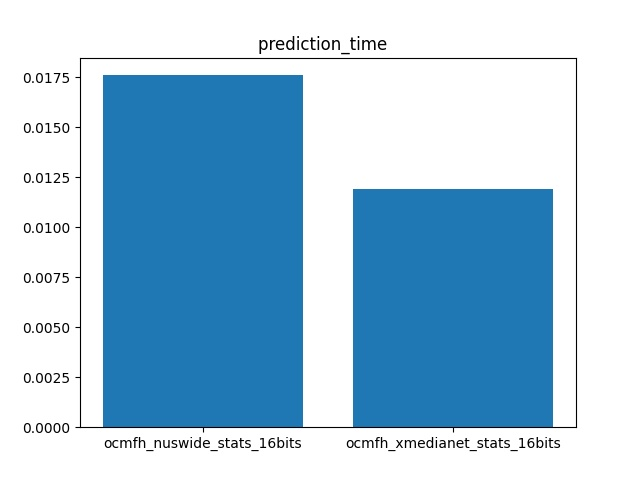
\includegraphics[width=\linewidth]{resultsImages/time/prediction_time_ocmfh_both.jpeg}
                % \caption{Inter comparison(NUS-WIDE)}
                % \label{fig:}
                \vspace{0.1ex}
                \hspace{0.1ex}
            \end{minipage}
            \begin{minipage}[!h]{0.6\linewidth}
                \centering
                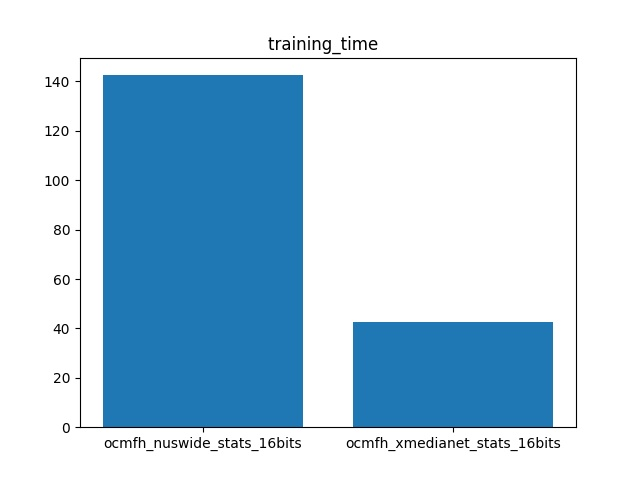
\includegraphics[width=\linewidth]{resultsImages/time/training_time_ocmfh_both.jpeg}
                % \caption{OCMFH chaning bits(Xmedianet)}
                % \label{fig:}
                \vspace{0.1ex}
                \hspace{1ex}
            \end{minipage}
            \begin{minipage}[!h]{0.8\linewidth}
                \centering
                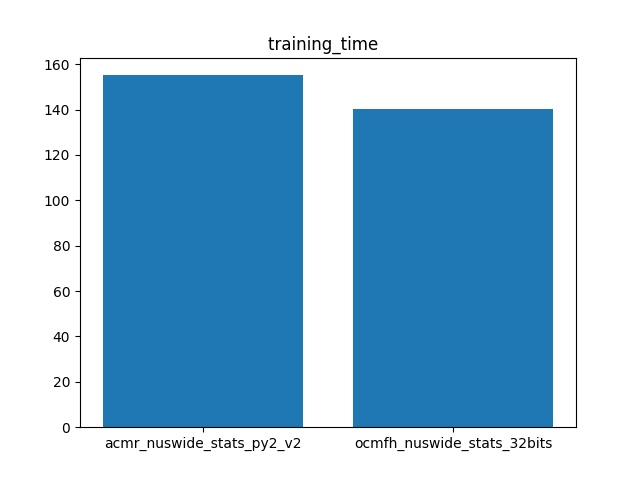
\includegraphics[width=\linewidth]{resultsImages/time/training_time _both_nuswide.jpeg}
                % \caption{OCMFH changing bits(NUS-WIDE)}
                % \label{fig:}
                \vspace{0.1ex}
                \hspace{0.1ex}
            \end{minipage}
            \caption{Training and prediction time for inter and intra method comparison on various datasets}
        \label{fig:}
        \end{figure}
        \FloatBarrier